\documentclass[tikz,border=7pt]{standalone}
\usepackage{iftex}
\ifPDFTeX
  \PackageError{matrix-figure}{This figure requires XeTeX or Tectonic}{Compile with xelatex or tectonic.}
\fi
\usepackage{fontspec}
\usepackage{xeCJK}
\usepackage{amsmath}
\usepackage{unicode-math}
\usepackage{xcolor}
\usepackage{tikz}
\usetikzlibrary{arrows.meta,positioning}

\providecommand{\FigureUseLocalFonts}{0}
\ifnum\FigureUseLocalFonts=1
  \setmainfont{NotoSansCJKtc-Regular.otf}[Path=\FigureSansFontPath]
  \setsansfont{NotoSansCJKtc-Regular.otf}[Path=\FigureSansFontPath,BoldFont=NotoSansCJKtc-Bold.otf]
  \setCJKmainfont{NotoSansCJKtc-Regular.otf}[Path=\FigureSansFontPath]
  \setCJKsansfont{NotoSansCJKtc-Regular.otf}[Path=\FigureSansFontPath,BoldFont=NotoSansCJKtc-Bold.otf]
  \setmathfont{STIXTwoMath.otf}[Path=\FigureMathFontPath]
\else
  \setmainfont{Noto Sans CJK TC}
  \setsansfont{Noto Sans CJK TC}
  \setCJKmainfont{Noto Sans CJK TC}
  \setCJKsansfont{Noto Sans CJK TC}
  \setmathfont{STIX Two Math}
\fi

\definecolor{FigureInk}{HTML}{253142}
\definecolor{PanelFill}{gray}{0.96}
\definecolor{RowShade}{gray}{0.86}
\definecolor{ColumnShade}{gray}{0.74}
\definecolor{ResultShade}{gray}{0.58}
\definecolor{FocusShade}{gray}{0.68}
\definecolor{GuideShade}{gray}{0.80}

\newcommand{\MatrixCell}[2]{%
  \tikz[baseline=(value.base)]{\node[fill=#1,rounded corners=0.4pt,inner sep=2.2pt,
    minimum width=1.35em,minimum height=1.35em] (value) {$#2$};}%
}
\newcommand{\RowCell}[1]{\MatrixCell{RowShade}{#1}}
\newcommand{\ColumnCell}[1]{\MatrixCell{ColumnShade}{#1}}
\newcommand{\ResultCell}[1]{\MatrixCell{ResultShade}{#1}}
\newcommand{\FocusCell}[1]{\MatrixCell{FocusShade}{#1}}

\tikzset{
  figure/.style={font=\sffamily,text=FigureInk,>={Stealth[length=3.5mm,width=2.5mm]}},
  panel/.style={draw=FigureInk,line width=0.9pt,rounded corners=1.5mm,fill=PanelFill,align=center},
  flow/.style={-{Stealth},line width=1.05pt,draw=FigureInk},
}


\begin{document}
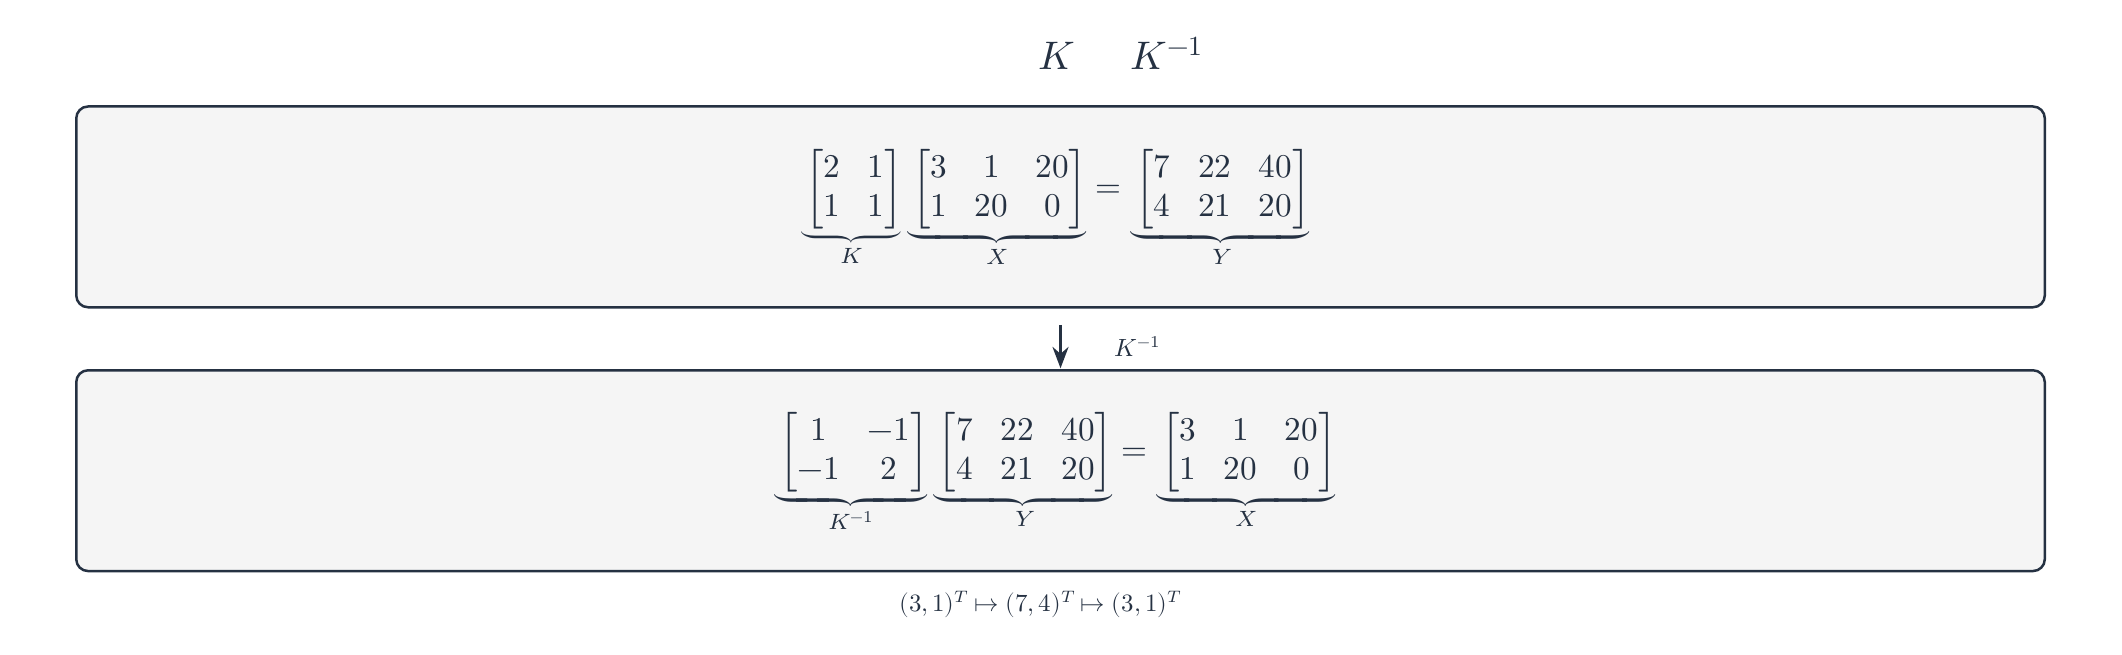
\begin{tikzpicture}[figure]
  \node[font=\bfseries\Large,align=center,text width=26cm] at (13,7.0)
    {每個資料直行先左乘可逆矩陣 $K$，再左乘 $K^{-1}$ 復原};

  \node[panel,minimum width=25.0cm,minimum height=2.55cm] at (13,5.05) {%
    \large
    $\underbrace{\begin{bmatrix}2&1\\1&1\end{bmatrix}}_{K}
     \underbrace{\begin{bmatrix}3&1&20\\1&20&0\end{bmatrix}}_{X}
     =\underbrace{\begin{bmatrix}7&22&40\\4&21&20\end{bmatrix}}_{Y}$
  };

  \draw[flow] (13,3.55) -- (13,3.0)
    node[midway,right,font=\small] {接收端左乘 $K^{-1}$};

  \node[panel,minimum width=25.0cm,minimum height=2.55cm] at (13,1.7) {%
    \large
    $\underbrace{\begin{bmatrix}1&-1\\-1&2\end{bmatrix}}_{K^{-1}}
     \underbrace{\begin{bmatrix}7&22&40\\4&21&20\end{bmatrix}}_{Y}
     =\underbrace{\begin{bmatrix}3&1&20\\1&20&0\end{bmatrix}}_{X}$
  };

  \node[font=\small] at (13,0.0)
    {第一筆資料：$(3,1)^T\mapsto(7,4)^T\mapsto(3,1)^T$；其餘直行使用同一規則。};
\end{tikzpicture}
\end{document}
